% \subsection{Satisfaction rate statistics generation algorithm}
% \label{sec:stats}

Statistic generation is performed at different time and name prefix granularities.  
% Figure~\ref{fig:stats tree} shows an overall design of the implemented statistics generation module and Pseudocodes~\ref{algo:loadstats}, \ref{algo:interest stats}, \ref{algo:prefix stats}, \ref{algo:stats} show implementation details.

% \begin{figure}[htpb]
%   \centering
%   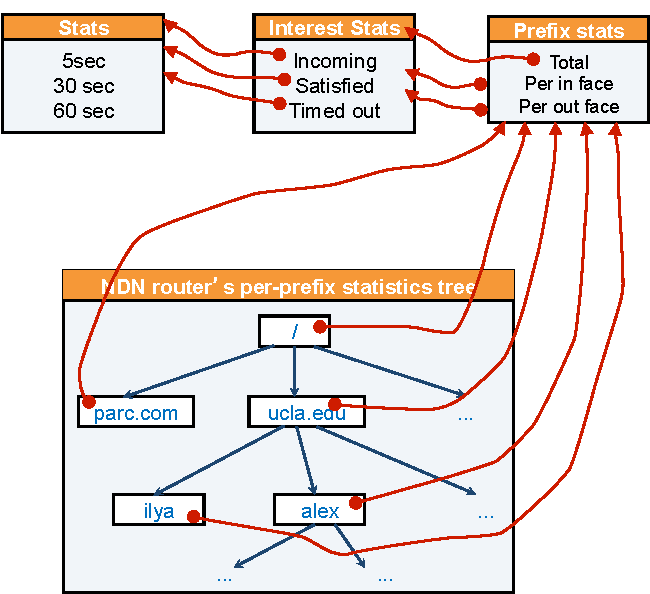
\includegraphics[scale=0.7]{figures/stats-illustration.pdf}
%   \caption{Statistics tree}
%   \label{fig:stats tree}
% \end{figure}


% A separate set of statistical information is kept for each Interest name, as well as aggregated to all Interest name prefixes, including root (``/'') prefix (per-prefix statistics tree on Figure~\ref{fig:stats tree}).

\floatname{algorithm}{Pseudocode}

%%%%%%%%%%%%%%%%%%%%%%%%%%%%%%
%%%%%%%%%%%%%%%%%%%%%%%%%%%%%%
%%%%%%%%%%%%%%%%%%%%%%%%%%%%%%

\begin{algorithm}[h]
\caption{Interest satisfaction statistics}
\label{algo:interest stats}
\begin{algorithmic}[1]

\vspace{0.2cm}

\For{\textbf{each} interface \em{if}}
    \State $F_{if} \leftarrow 0$ \Comment{forwarded Interests from interface \textbf{if}}
    \State $\hat F_{if} \leftarrow 0$ \Comment{averaged value of $F_{if}$}

    \State $U_{if} \leftarrow 0$ \Comment{unsatisfied Interests from interface \textbf{if}}
    \State $\hat U_{if} \leftarrow 0$ \Comment{averaged value of $U_{if}$}
\EndFor

\vspace{0.2cm}
\Function{OutInterest}{Interest \textbf{i}, InInterface \textbf{if}}
  \State $F_{if} \leftarrow F_{if} + 1$
  \State record \textbf{\emph{if}} in the list of incoming interfaces for \textbf{\emph{i}}
\EndFunction

\vspace{0.2cm}
\Function{InterestTimeout}{Interest \textbf{i}}
    \State lookup the list of incoming interfaces for \textbf{\emph{i}}

    \For{\textbf{each} interface $if$ in the list}
        \State $U_{if} \leftarrow U_{if} + 1$
    \EndFor
\EndFunction

\vspace{0.2cm}

\State {} \Comment{\textit{Exponential weighted moving average smoothing}}
\Function{EWMA}{} \Comment{Every second}
\State $\alpha \leftarrow e^{-1.0/30.0}$  %\Comment{$\approx$ 30~sec average}

\For{\textbf{each} interface \em{if}}
    \State $\hat F_{if} \leftarrow \alpha \cdot \hat F_{if} + (1 - \alpha) \cdot I_{if}$ 
    \State $\hat U_{if} \leftarrow \alpha \cdot \hat U_{if} + (1 - \alpha) \cdot U_{if}$ 

    \State $F_{if} \leftarrow 0$ \Comment{Reset counters}
    \State $U_{if} \leftarrow 0$ 
\EndFor

\EndFunction

\end{algorithmic}
\end{algorithm}

%%%%%%%%%%%%%%%%%%%%%%%%%%%%%%
%%%%%%%%%%%%%%%%%%%%%%%%%%%%%%
%%%%%%%%%%%%%%%%%%%%%%%%%%%%%%

% \begin{algorithm}[h]
% \caption{Prefix stats component}
% \label{algo:prefix stats}
% \begin{algorithmic}[1]



% \vspace{0.2cm}
% \Function{Advance}{} \Comment{Every second}
% \State $T.$advance()
% \For{\textbf{each} Face $f$}
%     \State $Stats[iface].$advance()
% \EndFor

% \EndFunction

% \end{algorithmic}
% \end{algorithm}

%%%%%%%%%%%%%%%%%%%%%%%%%%%%%%
%%%%%%%%%%%%%%%%%%%%%%%%%%%%%%
%%%%%%%%%%%%%%%%%%%%%%%%%%%%%%

% \begin{algorithm}[h]
% \caption{Statistics generation algorithm}
% \label{algo:stats}
% \begin{algorithmic}[1]

% \State stats $\leftarrow$ empty tree of Prefix stats \Comment{Stats tree}

% \vspace{0.2cm}
% \Function{ProcessEvent}{new Interest, inFace}
%   \State stats[Interest.Name].NewPitEntry()
%   \State stats[Interest.Name].Incoming(inFace);
%   \State stats[Interest.Name].Timeout()
% \EndFunction

% \vspace{0.2cm}
% \Function{ProcessEvent}{Interest rejected, inFace}
%   \State stats[Interest.Name].NewPitEntry()
%   \State stats[Interest.Name].Incoming(inFace)
% \EndFunction

% \vspace{0.2cm}
% \Function{ProcessEvent}{Interest forwarded, outFace}
%   \State stats[Interest.Name].Outgoing(outFace)
% \EndFunction

% \vspace{0.2cm}
% \Function{ProcessEvent}{pending Interest timeout}
%   \State stats[Interest.Name].Timeout()
% \EndFunction

% \vspace{0.2cm}
% \Function{ProcessEvent}{pending Interest satisfied}
%   \State stats[Interest.Name].Satisfy()
% \EndFunction

% \vspace{0.2cm}
% \Function{Periodic}{every second}
% \For{every node, walking from children to root}
%     \State $node.parent.$Combine($node$)
%     \State $node.$Advance()
% \EndFor
% \EndFunction


% \end{algorithmic}
% \end{algorithm}

\begin{figure}[htbp]
  \centering
  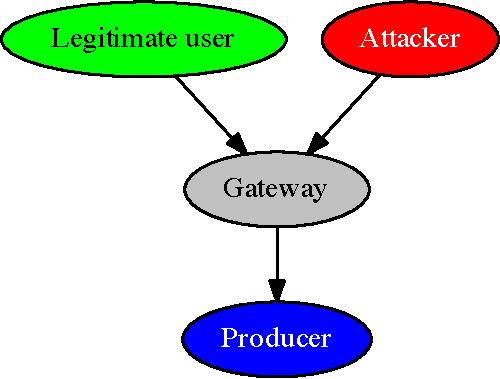
\includegraphics[width=4.5cm]{trivial-topo}
  \caption{Trivial topology (all links are 3Mbps/10ms)}
  \label{fig:trivial topology}
\end{figure}


\begin{figure}[htbp]
  \centering
  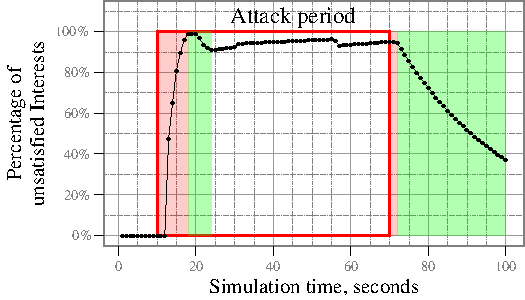
\includegraphics[scale=1]{limits}
  \caption{Dynamics of the unsatisfied Interests statistics on gateway's interface towards the attacker}
  \label{fig:ratio example}
\end{figure}


%%% Local Variables: 
%%% mode: latex
%%% TeX-master: "../paper"
%%% End: 
